\documentclass{amia}
\usepackage{graphicx}
\usepackage[labelfont=bf]{caption}
\usepackage[superscript,nomove]{cite}
\usepackage{color}
\usepackage{multirow}


\begin{document}


\title{Leverage machine learning methods for the classification of clinical interview fragment sequences}

\author{Mehedi Hasan, BS$^{1}$, Alexander Kotov, PhD$^{1}$, April Carcone, PhD$^{2}$, Sylvie Naar-King, PhD$^{2}$}

\institutes{
$^1$Department of Computer Science,  
$^2$Pediatric Prevention Research Center, Wayne State University, Detroit, Michigan\\
}

\maketitle

\noindent{\bf Abstract}
\textit{This study examines the effectiveness of state-of-the-art supervised machine learning methods for the task of automatic annotation of fragments of clinical interviews in conjunction with sequential analysis of that annotation. We used a collection of motivational interview transcripts consisting of 11,353 utterances, which were manually annotated by two human coders as a golden standard, and experimented with state-of-art classifiers, including Na\"{i}ve Bayes, J48 Decision Tree, Support Vector Machine (SVM), Random Forest (RF), AdaBoost, DiscLDA, Conditional Random Fields (CRF) and Convolutional Neural Network (CNN) in conjunction with lexical, contextual (label of the previous utterance) and semantic (distribution of words in the utterance across the Linguistic Inquiry and Word Count dictionaries) features. We found out that, when the number of classes is large, the performance of the CNN and CRFs is inferior to SVM. Among all classifiers using only lexical features, SVM achieved the highest classification accuracy of 70.8\%, 61\% and 53.7\%, when interview transcripts were annotated with the codebooks consisting of 17, 20 and 41 codes, respectively. Using contextual and semantic features, as well as their combination, in addition to lexical ones improved the accuracy of SVM for annotation of utterances in motivational interview transcripts with a codebook consisting of 17 classes to 71.5\%, 74.2\% and 75.1\%, respectively. We also used first order markov model that achieved 68.03\% accuracy for the classification of sequence of behavioral codes extracted from the above dataset. Therefore, our results demonstrate the potential of using machine learning  and textual data mining methods in conjunction with semantic and contextual features for automatic annotation of clinical interview transcripts  and their sequences with near-human accuracy.}


\section*{Introduction}
In this study, our analysis have two directions: automatic annotation and sequential data analysis. Annotation (or labeling) of fragments of clinical text with the categories (or labels, codes) from a predefined codebook is an integral part of qualitative research. It can also be viewed as classification of textual fragments into a predefined number of categories (classes). Textual annotation has been traditionally performed manually by trained coders, which is a tedious, costly and time-consuming process. Furthermore, manual annotation increases the likelihood of errors due to coder fatigue and bias associated with human subjectivity. To automate tedious cognitive tasks such as classification, supervised machine learning methods have been recently proposed. Although these methods have been shown to be successful at binary (two-class) classification \citep{40,41} (e.g. classifying textual fragments as neutral or opinionated), we are not aware of any prior studies reported in the literature that evaluate their performance for textual classification tasks involving large number of classes. Such tasks, however, are fairly common in clinical setting (e.g. annotation of clinical interviews, assignment of ICD-9/10 codes to patient records). To address this limitation, in this paper we propose contextual and semantic features and present the results of an extensive experimental evaluation of state-of-the-art supervised machine learning methods in conjunction with lexical and the proposed features for the task of automatic annotation of utterances in clinical interview transcripts with the codebooks consisting of large number of classes. Our study provides a guideline for clinical informatics researchers and practitioners, who consider an option of using machine learning methods for automatic annotation of clinical text in their projects.

Annotation of clinical interview transcripts to distinguish different behavior types is an important part of clinical research aimed at designing effective interventions for many conditions and disorders. In this paper, we focus on the transcripts of Motivational Interviews with obese adolescents (teens) and their caregivers. Childhood obesity is a serious public health concern in the United States and worldwide. Recent estimates indicate that approximately one third (31.8\%) of US children age 2-19 years are overweight and 16.9\% are obese \citep{01}. Adolescents who are obese are likely continue to be obese in adulthood and have a greater risk of heart disease, type 2 diabetes, stroke, cancer, and osteoarthritis \citep{02}. Therefore, there is a need for informatics-based methods to facilitate development of effective interventions for childhood obesity. One approach to designing intervention is Motivational Interviewing (MI), an evidence-based counseling technique to increase intrinsic motivation and self-efficacy for health-related behavior change \citep{03,04}. The goal of a MI counseling session is to encourage patients to explore their own desires, ability, reasons, need for and commitment to the targeted behavior change. These statements, referred to as ``change talk'' (or CT), consistently predict actual behavior change \citep{05} that can be sustained for as long as 34 months after an interview \citep{06}. The process of establishing causal linkages to identify effective communication strategies for eliciting change talk and commitment language in MI involves a resource-intensive qualitative coding process. First, clinical interviews are transcribed and then each utterance is manually annotated with a set of codes from a pre-defined codebook designating specific behavior types. Training human coders to reliably and accurately assign codes to textual fragments requires a large investment of manpower, time and money. For example, in a recent MI study \citep{07}, training coders to reliability took about four months and, once trained, coders required five hours to code every recorded hour. A similar study reported requiring 60 hours of training over six weeks to attain coder reliability, and the actual coding involved two coding passes and six coders \citep{08}.

Automatic annotation of patient utterances in clinical communication is a challenging task, since patients usually come from a variety of cultural and educational backgrounds and
their language use can be quite different \citep{09}. This problem is exacerbated when the interviews are conducted with children and adolescents due to their tendency to use
incomplete sentences and frequently change subjects.

Previous quantitative studies of clinical conversation have resulted in creation of Generalized Medical Interaction Analysis System (GMIAS) \citep{10}, which uses a codebook with generic hierarchical categories. The small-size codebook in Comprehensive Analysis of the Structure of Encounters System (CASES) \citep{11} was designed to annotate several
meta-discursive aspects of medical interviews, such as assigning ``ownership'' of topics and partitioning them into distinct segments (speech acts). It was also shown that the
fragments of transcripts of routine outpatient visits consisting of several speech acts coded using GMIAS and CASES can be annotated as ``information giving'' and ``requesting
information'' \citep{12}. Other related previous studies focused on categorizing assertions of medical problems in clinical narrative into 5 classes (present, absent, possible,
hypothetical, conditional and associated with someone else) using SVM \citep{13} and annotating the utterances in hemodialysis phone dialogue with 3 categories using AdaBoost
classifier \citep{14}. The present study reports the results of comprehensive evaluation of 8 state-of-the-art classifiers (Na\"{i}ve Bayes \citep{15,16,17}, Support Vector Machine
\citep{18,19}, Conditional Random Fields \citep{21,22}, J48 \citep{23}, AdaBoost \citep{24}, Random Forest \citep{42}, DiscLDA \citep{25} and Convolutional Neural Network
\citep{38}) for the task of annotating clinical interviews with a codebook, consisting of a large number of classes. We also propose and experimentally evaluate two novel features
for this task: contextual features based on the label of the preceding textual fragment and semantic features based on the distribution of words in the annotated fragment over a linguistic lexicon.

Codes automatically assigned to transcripts using classification models presented above allow to abstract away from the raw text  of the interviews and unequivocally establish the casual relationship between provider communication and client change talk (CT). Two recent studies \citep{46,47} have examined causality in treatment communication sequences using sequential analysis techniques to assess the probability that CT actually follows specific provider behaviors. Both studies found that provider use of MICO communication behaviors was followed by CT more frequently than expected and followed by client counter-CT (CCT; client statements against making changes) less frequently than expected by chance. Again, while suggestive of important PPC sequences, these studies were conducted among adults in treatment for alcohol abuse. In this project, we used a probabilistic model, in particular, first order markov model for the analysis of sequential data to determine provider-patient communication sequences that are likely to translate into change talk and commitment language.

\section*{Methods}
\subsection*{\textit{Data collection}}
The golden standard for evaluation of machine learning methods was created based on the transcripts of motivational interviews conducted by the clinicians at the Pediatric
Prevention Research Center (PPRC) of Wayne State University. Each interview is comprised of two parts: conversation of a clinician with an adolescent followed by a conversation of
a clinician with the adolescent's caregiver. All adolescents in this study were between the ages of 12 and 17 (M = 14.7, SD = 1.63) and most were female (n = 27). Most caregivers
were biological mothers (n = 36), who were married or living with a partner (n = 25). The median family income was \$16,000--\$21,999 ranging from less than \$1,000 to
\$50,000--\$74,999. The audio recordings of the interviews were first transcribed and segmented into utterances belonging to adolescents, caregivers, and counselors, preserving the
sequence of utterances. Transcripts were then manually annotated by trained human coders according to MYSCOPE \citep{07}, a specialized codebook including a large number of
behavior codes, which was developed by an interdisciplinary team including a clinical psychologist, a nutrition scientist, a communication scientist, a linguist and a community
health worker specifically for annotating motivational interviews with obese adolescents. A primary coder independently coded interview sessions and a secondary coder co-coded a
randomly selected 20\% of the transcripts to monitor reliability ($\kappa$ = 0.696) \citep{07}. The MYSCOPE codebook contains a total of 115 different codes that are grouped into
the youth, caregiver, and counselor code groups. The experimental datasets for this work were constructed based on the transcripts of 37 motivational interview sessions, which
include a total of 11,353 segmented and annotated utterances. These utterances have been further partitioned into two subsets based on the structure of motivational interview
sessions: one dataset that includes all utterances from the adolescent sessions (6,579 samples) and the other dataset that includes all utterances from the caregiver sessions
(4,774 samples). A fragment of an adolescent session transcript is presented in Table~\ref{table:06}.

\begin{table*}[htb]
\caption{\textbf{Fragment of the annotated transcript of a dialogue between a counselor and an adolescent.}}    
\label{table:06}
\centering
\begin{tabular}{lp{3.6cm}lp{8cm}}
\hline
\hline
Annotation  & Description & Speaker & Text \\
\hline
331 &	Open-ended question, elicit change talk positive &	Counselor &	do you feel like making healthier choices for your snacks and your meals is something you would be able to do ? mm-hmm meaning is that food available for you ? \\
117 &	Low Uptake, positive	& Adolescent &	Yes \\
301 &	Structure Session	& Counselor &	okay and thats an important thing for us to think about cause i would not want to help you come up with a plan that you would not be able to do without somebody else help so the last part of your plan is how somebody could be supportive to you meaning how they can help you be successful and so we should choose somebody who you feel like is around often enough \\
112 &	Change Talk positive	& Adolescent &	my um aunt \\
301 &	Structure Session	& Counselor &	okay so lets stick something my aunt can do \\
112 &	Change Talk positive &	Adolescent &	she could when i am doing when i am eating something that i should i could not be eating but so i can choose something healthy she could tell me not to eat it \\
309 &	Affirm, low &	Counselor &	okay that sounds like a really great suggestion \\
\hline
\hline
\end{tabular}
\end{table*}

To conduct a detailed analysis of performance of classification methods, we used the following two-stage process to create the codebooks with different number of codes for
adolescent and caregiver sessions. In the first stage, we merged conceptually similar behavior codes as well as the codes with similar data distributions, while in the second stage, we eliminated the codes with insufficient data samples. In case of the adolescent sessions, we started with 55 adolescent session-specific codes and, after merging the codes with subtle differences (e.g. converting valiances of change talk CHT+1, CHT+2 and CHT+3 into CHT+), obtained a codebook with 41 classes. We further reduced this codebook to 20 classes after merging 21 classes with similar sample distributions. After eliminating the codes that had less than 10 data samples (to ensure that there can be at least one sample of each class in each fold when using 10-fold cross validation experimental design), we obtained a third codebook with 17 codes. Using the same approach, we created the codebooks containing 58, 19, and 16 caregiver session-specific codes. Table~\ref{table:01} shows the distribution of utterances over 16 classes in the caregiver session transcripts. As follows from Table~\ref{table:01}, the distribution of utterances over classes is highly imbalanced even for the codebook of the smallest size, which is fairly common for clinical text. To create the gold standard for our second experiment, we partitioned the adolescent transcripts into sequence of successful and unsuccessful codes which are ended with either negative or positive change talk and commitment language. Table~\ref{table:0001} depicts the distribution of PPC code sequences over the adolescent dataset.

After creating the codebooks, we pre-processed the dataset using the Snowball stemmer available as part of the Weka \citep{26} machine learning toolkit\footnote{
http://www.cs.waikato.ac.nz/ml/weka/}. We also found out that stopword removal decreased the performance of classification models for our task (e.g., in case of the codebook
consisting of 17 classes, the accuracy of Na\"{i}ve Bayes decreased from 67\% to 47.10\%, while the accuracy of SVM decreased from 70.76\% to 55.26\%). A likely reason is that,
although negations are typically considered as stopwords, they are fairly important clues for inferring certain behavior types (e.g., removing the stopword ``not'' completely
transforms the meaning of a phrase ``not great'').

\subsection*{\textit{System overview}}
The pipeline consists of two stages: training and testing. Prior to the training stage, we preprocess the collected clinical interview transcripts by performing stemming, punctuation removal, word segmentation and tokenization. Features are then extracted from the preprocessed data. During this stage, previous label and LIWC features are used in conjunction with the lexical features to create the feature vectors. After that, classifiers are trained on the feature vectors extracted from the training samples and their associated annotations. In the testing stage, after creation of feature vectors, the previously trained classifiers predict the label of each utterance in the testing sample. Finally, performance of different classifiers is evaluated by calculating standard metrics such as precision, recall, F-score (F1), kappa measure and accuracy. Specifically, we evaluated the performance of the following state-of-the-art supervised machine learning methods.

\textbf {Markov Model}: In probability theory, a markov model \citep{45} is a stochastic model used to model randomly changing systems where it is assumed that future states depend only on the present state and not on the sequence of events that preceded it (that is, it assumes the markov property). Generally, this assumption enables reasoning and computation with the model that would otherwise be intractable. For the sequential analysis, we built two markov models $M$ and $\overline{M}$ describing provider strategies and patient responses in case of successful ($M$) and unsuccessful ($\overline{M}$) motivational interviews. A markov model $M$ can be represented as a weighted directed graph $G = (V, E, p)$, in which:

\begin{itemize}
\item $V = \{CML+, CHT+, CHT-, T-AMB, CCT, BLT, LUP+, LUP-, HUP-W, ...\}$ is a set of vertices, consisting of possible youth and counselor MI behavior codes;
\item $E \subseteq V \times V$ is a set of edges corresponding to posssible transitions from one MI behavior code to the other in a sequence;
\item $p_M:E\rightarrow[0...1]$ is a function that assigns probability $p(c_i|c_j)$ to an edge between the MI behavior codes $c_i$ and $c_j$ based on maximum likelihood estimator:

\begin{equation}
P_M(c_j|c_i) = \frac{n_{c_i,c_j}}{n_{c_i}}
\end{equation}

\end{itemize}

where $n_{c_i,c_j}$ and $n_{c_i}$ are the number of times a transition between the MI behavior codes $c_i$ and $c_j$ and the code $c_i$ have been observed in the training data. Given a markov model $M$ (such that $S\subseteq V$), a sequence of MI behavior codes $S = \{C_1,...,C_N\}$ have been generated from a markov model $M$ is:

\begin{equation}
P_M(S) = \prod_{i=2}^N p_M(c_i|c_1,\dots,c_{i-1})=\prod_{i=2}^N p_M(c_i|c_{i-1})
\end{equation}

Success of a given motivational interview, given a sequence of MI behavior codes corresponding to it, can be predicted based on the following formula:

\begin{equation}
p(S\rightarrow CT) = \log\left(\frac{P_M(S)}{P_{\overline M}(S)}\right)= \sum_{i=2}^N p_M(c_i|c_{i-1})-\sum_{i=2}^N p_{\overline M}(c_i|c_{i-1})
\end{equation}

if $p(S\rightarrow CT) > \delta $, where $\delta$ is experimentally defined threshold, the interview transcript (or a portion of it) is predicted to result in CT. We experimentally determined the value of $\delta$ to 0.3 which provides acceptable accuracy with minimum false positive rate. Figure\ref{fig:delta} illustrates the characteristics of proposed model by varying the value of $\delta$.  

\begin{figure}[htb!]
    \centering
    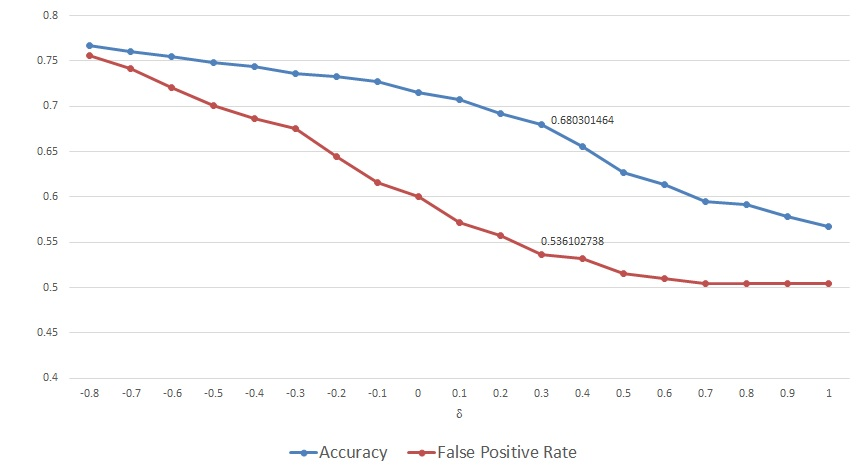
\includegraphics[width=0.70\textwidth]{figures/deltadata.jpg}
    \caption{\textbf{Characteristics of proposed markov model by varying the value of $\delta$}}
    \label{fig:delta}
\end{figure}

\subsection*{\textit{Evaluation methods}}
To ensure the robustness of performance estimates, we used 10-fold cross validation for the annotation of clinical interview fragments, and 5-fold cross validation for the classification of sequence of behavior codes \citep{36} as an experimental design. The performance of different classifiers and feature sets was evaluated in terms of precision, recall, F1 score (F1), kappa measure and accuracy using weighted macro-averaging over folds.

\section*{Results}
Experimental evaluation of automatic annotation of clinical interview fragments and their sequences by using machine learning and probabilistic model included several dimensions:
\begin{itemize}
\item determining the performance of classifiers on the codebooks of different size;
\item determining the effectiveness of the proposed contextual and semantic features.
\item determining the performance of markov model in conjunction with determining PPC sequences that are most likely to translate into CT.
\end{itemize}

Since clinical researchers typically annotate caregiver and adolescent sessions separately, we first created two experimental datasets consisting of only adolescent and only caregiver session transcripts. Second, besides evaluating the accuracy of annotating adolescent and caregiver transcripts with the codebooks containing an entire set of codes, we also conducted a series of experiments with the codebooks of smaller sizes created as outlined above. Third, besides training and testing NB, SVM, CRF, Decision Tree, Boosting, DiscLDA, Random Forest and CNN classifiers using only lexical features, we also evaluated the effectiveness of the proposed contextual and semantic features.

Depending on the type of the interview transcript and the codebook size, SVM-AF achieves 3\%--9\% higher accuracy and 4\%--10\% higher F1 score than SVM and 4\%--10\% higher accuracy and 4\%--11\% higher F1 score than CRF, which highlights the importance of contextual and semantic features.

\subsection*{\textit{Performance of Markov model in conjunction with determining PPC code sequences that are most likely translate into CT}}
Since clinical researchers tried to increase the desire and ability of adolescent to change their current behavior to target behavior, we used sequence of successful and unsuccessful codes only from adolescent session for our sequential analysis. Summary of performance for the classification of sequential data is presented in Table~\ref{table:sequence}. 
From Table~\ref{table:sequence}, it follows that our designed markov model works very well in terms of precision and achieves precision 0.7574 with F1-measure 0.7092. The strength of the model for the classification of each type of sequences is illustrated by providing the confusion matrix in Table~\ref{table:conf}. It also shows that successful patterns are identified more accurately compare to unsuccessful motivational interview sequences due to the imbalance of data.\\

\begin{table}[h]
\centering
\caption{Performance of markov models for the classification of normal PPC code sequence.}
\label{tab:result_norm_seq}
  \begin{tabular}{|l|l|l|l|l|l|}
  \hline
   \textbf{Model} & \textbf{Order}  & \textbf{Precision}  & \textbf{Recall} & \textbf{F-Measure} & \textbf{Accuracy}\\ \hline    
    
 \multirow{2}{*}{General Markov Chain} & First order & 0.7387 & 0.7686 & 0.7532 & 0.7686\\\cline{2-6}
 & Second order & 0.6889 & 0.7889 & 0.7352 & 0.7889\\ \hline
 \multirow{2}{*}{Hidden Markov Model} & First order & \textbf{0.7980} & 0.8059 & \textbf{0.7989} & 0.8059\\ \cline{2-6}
 & Second order & 0.7400 & \textbf{0.8449} & 0.7822  & \textbf{0.8449}\\ \hline
 
  \end{tabular}
\end{table}

\begin{table}[h]
\centering
\caption{Performance of markov models for the classification of alternate PPC code sequence.}
\label{tab:result_alt_seq}
  \begin{tabular}{|l|l|l|l|l|l|}
  \hline
   \textbf{Model} & \textbf{Order}  & \textbf{Precision}  & \textbf{Recall} & \textbf{F-Measure} & \textbf{Accuracy}\\ \hline    
    
 \multirow{2}{*}{General Markov Chain} & First order & 0.9777 & 0.9437 & 0.9604 & 0.9437\\\cline{2-6}
 & Second order & \textbf{0.9778} & 0.9694 & \textbf{0.9736} & 0.9694\\ \hline
 \multirow{2}{*}{Hidden Markov Model} & First order & 0.9392 & 0.9313 & 0.9253 & 0.9392\\ \cline{2-6}
 & Second order & 0.9704 & \textbf{0.9713} & 0.9699  & \textbf{0.9713}\\ \hline
 
  \end{tabular}
\end{table}

Two markov models are used to obtain top five most likely successful and unsuccessful motivational interviews that describing provider strategies and patient responses. Table~\ref{table:topsec} shows the top five successful and unsuccessful PPC code sequences.

\section*{Discussion}
From the sequential analysis, we observed that markov model achieved near-human accuracy to categorise the sequence of behavior codes. It was also found that successful interviews are more frequently responded by the adolescent with PPC code 112. However, unsuccessful interviews are responded with the behavior code 109.

\section*{Conclusion}
In this work, we suggest some successful sequences of codes for the practical use by the clinician during the interview session which will translate into positive change talk and commitment language. We also propose novel features and report the results of an extensive experimental evaluation of state-of-the-art supervised machine learning methods for text
classification using those features, to help clinical researchers and practitioners assess the feasibility of using these methods for the task of automatic annotation of clinical
text using the codebooks of realistic size. We found out that Support Vector Machine using only lexical features consistently outperforms all other classifiers on caregiver and
adolescent datasets according to most metrics. Adding contextual and semantic features further improves the performance of SVM on both datasets, achieving close to human accuracy
when the codebooks consisting of 16 and 17 classes are used to annotate caregiver and adolescent transcripts, respectively.

This work has important practical implications. First, it can facilitate researchers to establish causal relationship between different communication strategies and desired
behavioral outcomes without having to repeatedly wade through pages of interview transcripts. Second, since automatic annotation is significantly faster than manual, it can
dramatically accelerate the pace of research in behavioral sciences. Third, information that can directly inform and increase the efficiency of clinical practice for a successful interview. Although all experiments were conducted on interview transcripts, the proposed methods and features are not
specific to a particular domain of Motivational Interviewing, and thus there is also no prima facie reason to believe that they will not be effective for annotation of any other
type of clinical conversation.


\section*{Acknowledgments}
We would like to thank the technical staff at Henry Ford Health Systems and Textual Data Analytics Laboratory at Wayne State University for their help with collecting and transforming binary data into free text EHR used for experiments reported in this paper. 

\bibliographystyle{vancouver}
\bibliography{references}

\end{document}